\subsection{Raster datamodel} \label{Afsnit: Raster data model}

En rastermodel er en datamodel der er bygget op af et regulært netværk af celler organiseret i et gitterformat \citep{bolstad_gis_2022, esri_raster}. Hver celle i en raster model er karakteriseret af en celle dimension, som definerer cellestørrelsen ud fra cellens længde i X- og Y-retningen \citep{bolstad_gis_2022, silbernagel_raster_2018}. Cellestørrelsen repræsenterer således den rumlige opløsning af raster datamodellen og fungerer som en indikator for den rumlige præcision, da hver celles koordinat er givet ud fra centrum af cellen. En større cellestørrelse vil derfor resultere i en højere rumlig usikkerhed, mens en mindre cellestørrelse vil medføre en lavere rumlig usikkerhed \citep{bolstad_gis_2022}. \\

Hver celle i en raster indeholder en værdi, der repræsenterer information. Denne information kan enten kan være numerisk eller kategoriske. Numeriske værdier anvendes ofte til at repræsentere kontinuerlige data, såsom højdeinformationer i en højdemodel (figur \ref{Subfig: Kontinuer raster}), mens kategoriske værdier anvendes ved diskret og tematiske data, såsom arealklasser (figur \ref{Subfig: Kategorisk raster}). 
\begin{figure}[H]
    \begin{subfigure} [t]{0.5\textwidth}
        \centering
        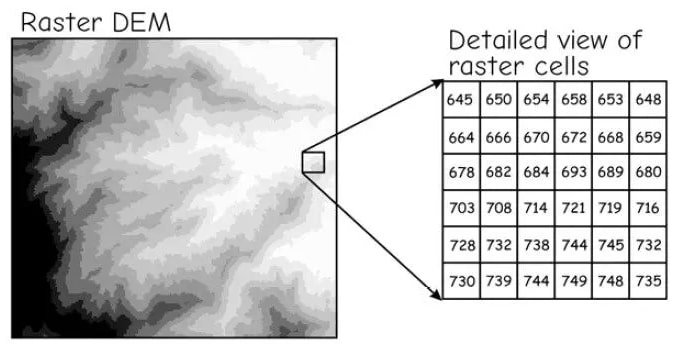
\includegraphics[width=1\linewidth]{images/teori/raster_kontinuert.jpg}
        \caption{}
        \label{Subfig: Kontinuer raster}
    \end{subfigure}
    \begin{subfigure} [t]{0.5\textwidth}
        \centering
        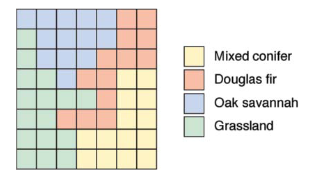
\includegraphics[width=1\linewidth]{images/teori/raster_areal.png}
        \caption{}
        \label{Subfig: Kategorisk raster}
    \end{subfigure}
    \caption{Eksempel på en raster med numeriske kontinuert data fra en højdemodel \textbf{(a)} og en kategorisk raster med diskrete data over arealanvendelse \textbf{(b)}. Kilde: \cite[s. 66]{bolstad_gis_2022} og \cite[s. 67]{longley_geographical_2008}}
    \label{Figur: Kontinuert og kategorisk raster}
\end{figure}

Rastermodellens struktur muliggør omfattende rumlig analyse, idet der kan udføres artimetiske og logiske operationer på tværs af celler og mellem flere forskellige rasterlag. Denne egenskab gør det derfor også muligt at analysere og kombinere kontinuerte og diskrete rumlige informationer i et GIS-miljø \citep{bolstad_gis_2022, longley_geographical_2008}.

\subsection{Inundation Modellen} \label{Afsnit: Inundation Model}

Til projektet er der blevet anvendt en GIS-baseret stormflods model kaldet \textit{"Inundation Model"} udarbejdet af \cite{balstrom_kirby_inundation} til at give et bud på hvordan en stormflod vil påvirke et område. Modellen opererer eksklusivt i et ArcGIS Pro miljø, GIS-softwaren udviklet af Esri.\\
Modellen indeholder en række værktøjer, der bruges til at analysere stormfloders påvirkning af et område og kernen i modellen er værktøjet \textit{"Create Inundation"} som er en statisk numerisk rastermodel. Modellen benytter tre brugerdefineret parametre der består af tre numeriske værdier i meter: InitialSealLevel, SeaLevelIncrement og Number of Iterations. Modellen benytter også en hydrologisk korrigeret Digital Terræn Model (DHyM) og en bruger digitaliseret linjeobjekt som kilde for udregningen, benævt Line at Sea \citep{balstrom_kirby_inundation}. I figur \ref{Figur: Create Inundation} er modellens opbygning vist inddelt i to segmenter.

\begin{figure}[H]
    \centering
    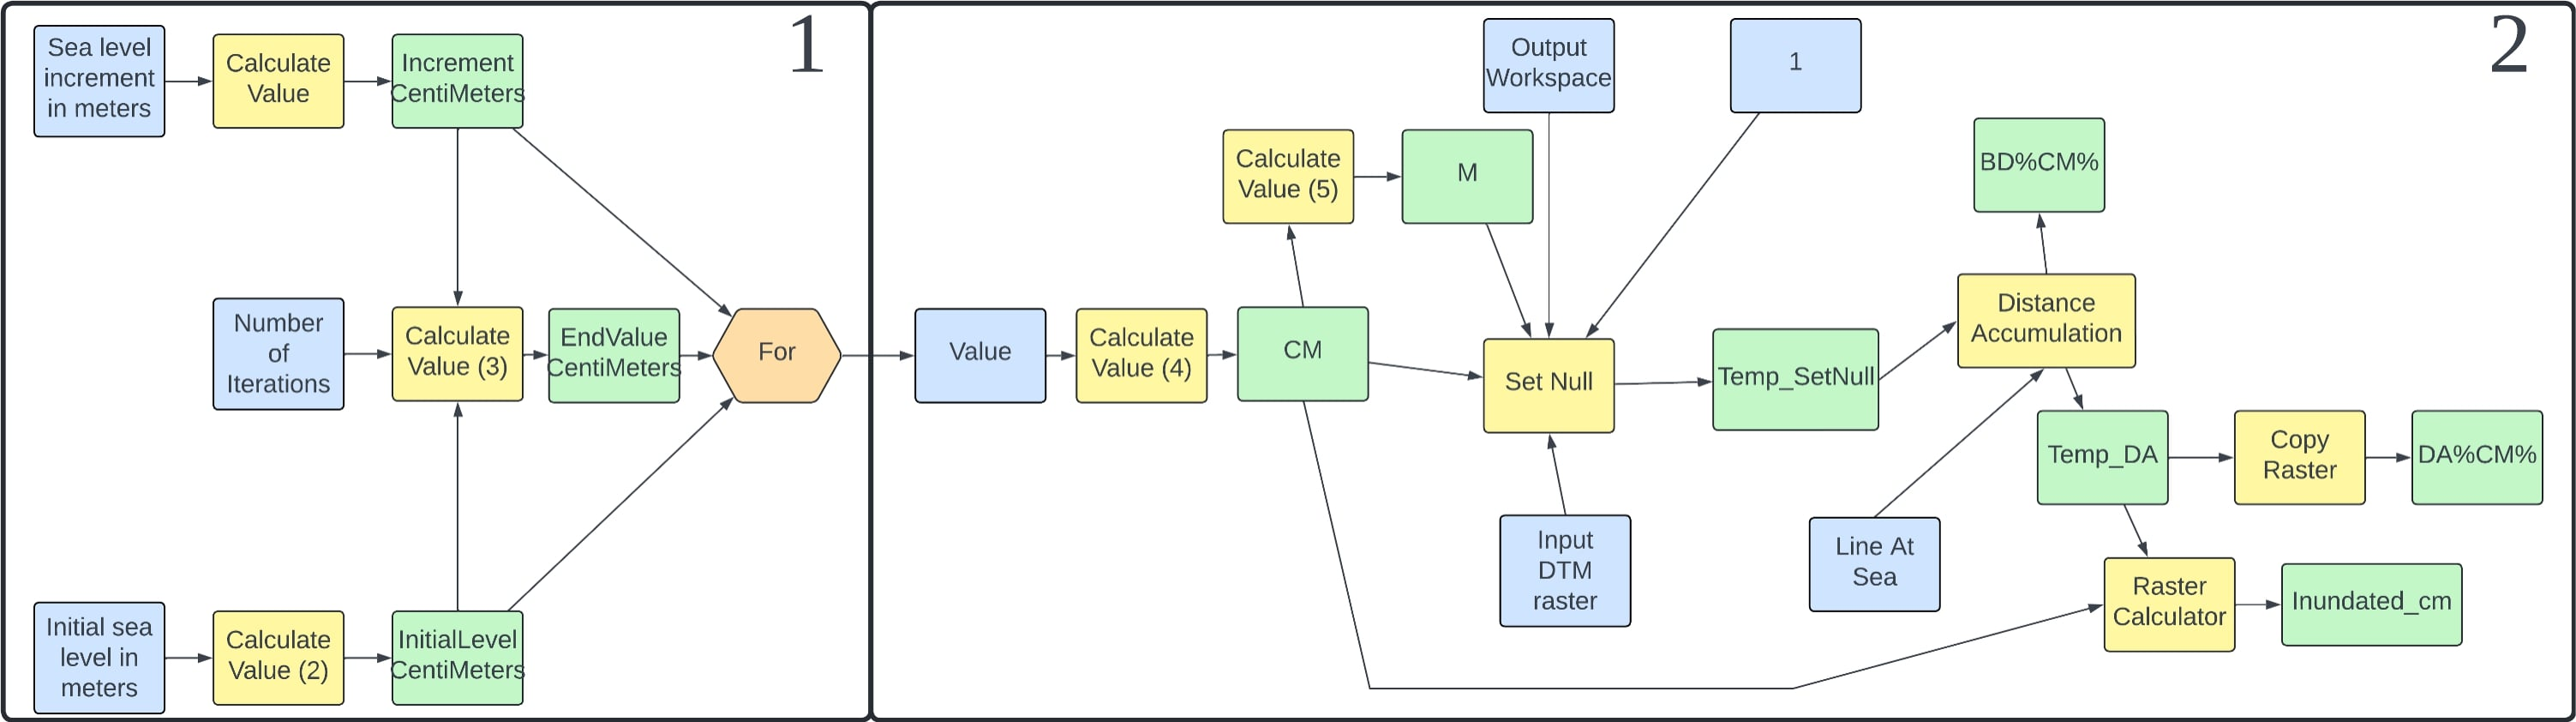
\includegraphics[width=1\linewidth]{images/teori/inundation_model_separated.jpg}
    \caption{Flowchart af Inundation Modellens \textit{"Create Inundation"} værktøj.}
    \label{Figur: Create Inundation}
\end{figure}

Det første segment er en omregning af brugerens input i meter til centimeter for både stigningsniveauet for hver gang modellen itererer og det begyndende havniveau. Modellen kræver en afsluttende værdi for hvornår den skal stoppe med at iterere. Denne værdi svarer til den vandstand der ønskes at simulere op til. Denne værdi bliver udregnet ved følgende: $InitialSeaLevel + ((NumberIterations - 1)\times Increment)$. \\

Det andet segment af modellen er selve oversvømmelses beregningen gennem terrænet. Det starter med et for-loop der starter med den første værdi (fx 100 cm). Denne værdi omregnes tilbage til meter hvorefter modellen eksekverer et tjek (figur \ref{Figur: Create Inundation} "SetNull") på cellerne i DTM. Her tjekkes alle celleværdierne i DTM for om de er større eller ligmed den nuværende værdi. Hvis dette hvis-ellers tjek er sandt bliver cellerne tildelt NoData værdien, som indikerer at cellen ikke bliver oversvømmet ved dette oversvømmelsesniveau. Hvis DTM celleværdien er lavere end tjekværdien og udtrykket dermed er falsk bliver cellen angivet med et 1, som indikerer at den bliver oversvømmet ved det niveau (figur \ref{Figur: Celler Inundated}).       

\begin{figure}[H]
    \centering
    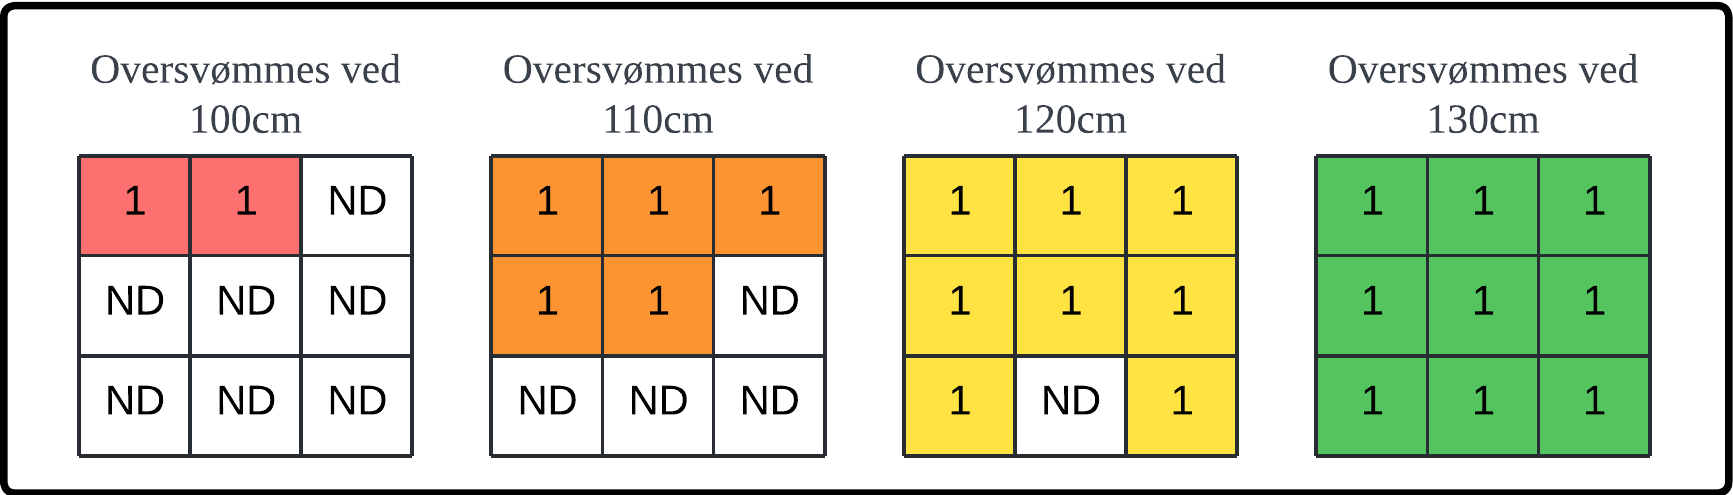
\includegraphics[width=0.7\linewidth]{images/teori/celler_inundated.png}
    \caption{Princippet bag Inundation Modellen gennem raster celler. 1 angiver at cellen oversvømmes ved det pågældende niveau og ND = NoData (celler som ikke bliver oversvømmet).  Egen illustration med inspiration fra \cite{balstrom_kirby_inundation}}.
    \label{Figur: Celler Inundated}
\end{figure}

Herefter udføres en Distance Accumulation igennem de celler der bliver oversvømmet ved det bestemte niveau fra en linjekilde. En Distance Accumulation er en analysemetode der beregner den samlede afstand fra en kilde ud igennem et område \citep{esri_how_nodate}. I Inundation modellen bliver Distance Accumulation brugt til at efterligne vandets bevægelse igennem cellerne på samme måde som vandet ville sprede sig under en stormflod. Distance Accumulation vil sprede sig igennem terrænet indtil en ufremkommelig barriere er mødt.\\ 
Distance Accumulation starter fra linjen \textit{"Line at Sea"} og bevæger sig igennem alle cellerne i terrænet hvor cellen = 1. Hvis cellen er NoData så kan vandet ikke bevæge sig igennem \citep{balstrom_kirby_inundation}. Resultatet af Distance Accumulationen bliver derefter koblet med det oversvømmelsesniveau der bliver itereret over for at give resultatet af modellen.  
